\documentclass{report}

% Language setting
% Replace `english' with e.g. `spanish' to change the document language
\usepackage[english]{babel}

% Set page size and margins
% Replace `letterpaper' with`a4paper' for UK/EU standard size
\usepackage[letterpaper,top=2cm,bottom=2cm,left=3cm,right=3cm,marginparwidth=1.75cm]{geometry}

%Code package
\usepackage{listings}
\lstdefinestyle{mystyle}{
    basicstyle=\ttfamily\footnotesize,
    breakatwhitespace=false,         
    breaklines=true,                 
    captionpos=b,                    
    keepspaces=true,                 
    numbers=left,                    
    numbersep=5pt,                  
    showspaces=false,                
    showstringspaces=false,
    showtabs=false,                  
    tabsize=2
}

\lstset{style=mystyle}

% Useful packages
\usepackage[export]{adjustbox}
\usepackage{amsmath}
\usepackage{graphicx}
\usepackage{enumitem}
\usepackage[colorlinks=true, allcolors=blue]{hyperref}

\title{Progetto di Business Intelligence per i Servizi Finanziari}
\author{Banfi Michele 869294}

\begin{document}
\maketitle

\chapter{Sommario dei dati utilizzati}
\section{Titoli}
I titoli scelti per questo progetto sono i seguenti:

\noindent Settore tecnologico

Netflix, Inc. (\textbf{NFLX})

Meta Platforms, Inc. (\textbf{META})

\noindent La scelta di Netflix é stata basata sulle notizie di questi ultimi anni della perdita di utenti e del raggiungimento di utenti massimi che Netflix ha riscontrato e il conseguente calo del titolo sul mercato. Mentre Meta é stata presa in considerazione per il recente cambio di brand e nome, da Facebook a Meta, successivo al lancio del Metaverso

\noindent Settore finanziario

The Goldman Sachs Group, Inc. (\textbf{GS})

Citigroup Inc. (\textbf{C})

\noindent Le scelte di queste due aziende sono dovuto al loro andamento dopo un calo, infatti Goldman Sachs, dopo il calo del covid si é subito ripresa e ha raddoppiato il suo valore in meno di un anno. Mentre Citigroup dopo la crisi finanziaria del 2008 non ha mai raggiunto di nuovo i valori che aveva precedentemente

\noindent Settore consumer defensive

The Coca-Cola Company (\textbf{KO})

PepsiCo, Inc. (\textbf{PEP})

Coca-Cola e PepsiCo sono stati scelti in quanto concorrenti allo stesso mercato e in quando non hanno subito un calo dopo il covid-19 e inoltre, il loro andamento nel mercato sembra essere costante in rialzo.

\section{Scaricare i dati}
Per prima cosa importiamo le librerie che ci serviranno in questo progetto:
\begin{lstlisting}[language=Python]
    import pandas as pd
    import numpy as np
    import matplotlib.pyplot as plt
    import yfinance as yf
\end{lstlisting}
Procediamo al dowload dei dati tramite \lstinline{yfinance.download()}
\begin{lstlisting}[language=Python]
    start = "2012-11-30"
    end = "2022-11-30"

    #Tech
    NFLX = yf.download("NFLX", start, end)
    META = yf.download("META", start, end)

    #Financials
    GS = yf.download("GS", start, end)
    C = yf.download("C", start, end)

    #Consumers
    KO = yf.download("KO", start, end)
    PEP = yf.download("PEP", start, end)
\end{lstlisting}
\section{Fusione dei dati}
Ora procediamo alla fusione dei dati in un unico DataFrame e di ogni titolo prendiamo solo l'"Adj close".
\begin{lstlisting}[language=python]
    market = pd.concat([NFLX['Adj Close'], META['Adj Close'], GS['Adj Close'], C['Adj Close'], KO['Adj Close'], PEP['Adj Close']], axis=1)
    market.columns = ['NFLX', 'META', 'GS', 'C', 'KO', 'PEP']
\end{lstlisting}
\section{Presentazione dei dati}
Per mostrare la struttura del nostro DataFrame possiamo usare la seguente funzione che ci ritorna le righe iniziali del nostro DataFrame
\begin{lstlisting}[language=python]
    market.head()
\end{lstlisting}
\begin{tabular}{lrrrrrr}
\toprule
{} &       NFLX &       META &          GS &          C &         KO &        PEP \\
Date       &            &            &             &            &            &            \\
\midrule
2012-11-30 &  11.672857 &  28.000000 &   99.521103 &  28.667482 &  27.682371 &  52.271511 \\
2012-12-03 &  10.857143 &  27.040001 &  100.036469 &  28.377247 &  27.288162 &  52.018406 \\
2012-12-04 &  12.378571 &  27.459999 &   98.498741 &  28.435295 &  27.120255 &  52.010952 \\
2012-12-05 &  11.910000 &  27.709999 &   98.963432 &  30.234777 &  27.237057 &  52.301300 \\
2012-12-06 &  12.310000 &  26.969999 &   99.022560 &  30.699169 &  27.288162 &  52.533886 \\
\bottomrule
\end{tabular}

E inoltre possiamo procedere anche alla stampa di un grafico di questi dati:
\begin{lstlisting}[language=python]
    market.plot(grid=True, title="Markets Adjs Closes")
    market.plot(grid=True, title="Markets Adjs Closes", subplots=True)
\end{lstlisting}

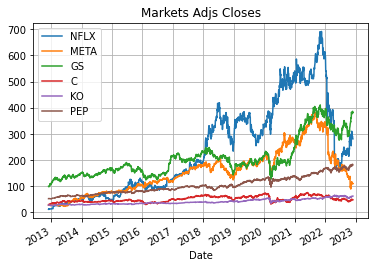
\includegraphics[width=0.5\textwidth, center]{market.png}

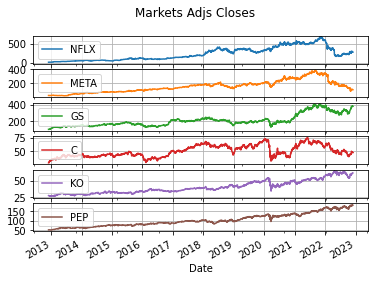
\includegraphics[width=0.5\textwidth, center]{marketSubplots.png}

\chapter{Statistiche descrittive}
\section{Rendimenti annauli}
Per calcolare il rendimento \textbf{composto} e \textbf{cumulato annuale} dobbiamo prima trasformare i dati da giornalieri ad annuali nel seguente modo:
\begin{lstlisting}[language=python]
    NFLXy = NFLX.groupby(pd.Grouper(freq='Y')).last()
\end{lstlisting}
Li raggruppiamo e li salviamo in \lstinline{marketY}.
Dopodiché possiamo procedere con il calcolo dei \textbf{rendimenti cumulati annui} e quello dei \textbf{rendimenti composti annui}:
\begin{lstlisting}[language=python]
    #Rendimento cumulato dei nostri titoli
    marketY2 = marketY.pct_change(1)
    marketY2 = marketY2.dropna()
    marketY3 = np.cumprod(marketY2 + 1)

    #Rendimento composto annuale NFLX
    rcoNFLXy = ((marketY['NFLX'][-1]/marketY['NFLX'][0])**(1/marketY['NFLX'].count()) - 1) *    100
\end{lstlisting}
Applichiamo questo procedimento per tutti i titoli.

\noindent Questo é il risultato dei nostri rendimenti cumulati:

\begin{tabular}{lrrrrrr}
\toprule
{} &       NFLX &      META &        GS &         C &        KO &       PEP \\
Date       &            &           &           &           &           &           \\
\midrule
2013-12-31 &   3.976347 &  2.052968 &  1.407936 &  1.318358 &  1.172331 &  1.246481 \\
2014-12-31 &   3.689491 &  2.930879 &  1.559786 &  1.370062 &  1.234067 &  1.461696 \\
2015-12-31 &   8.647370 &  3.931630 &  1.469481 &  1.314142 &  1.297496 &  1.589572 \\
2016-12-31 &   9.359542 &  4.321938 &  1.982669 &  1.523134 &  1.292863 &  1.713495 \\
2017-12-31 &  14.512582 &  6.628851 &  2.136010 &  1.934785 &  1.478803 &  2.018807 \\
\bottomrule
\end{tabular}

\section{Rendimenti semplici e logaritmici}
Usiamo le seguenti formule per calcolarci i \textbf{rendimenti semplici} e \textbf{logaritmici}
\begin{lstlisting}[language=python]
    #Rendimento semplice
    rsNFLX = NFLX['Adj Close'] / NFLX['Adj Close'].shift(1)
    #Rendimento logaritmico
    rlNFLX = np.log(NFLX['Adj Close'] / NFLX['Adj Close'].shift(1))
\end{lstlisting}
Applichiamo le stesse formule per tutti i titoli e li uniamo in un singolo DataFrame ottenendo i seguenti grafici

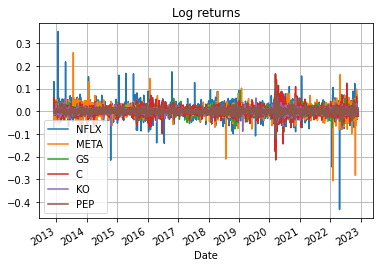
\includegraphics[width=0.5\textwidth, center]{logReturns.png}

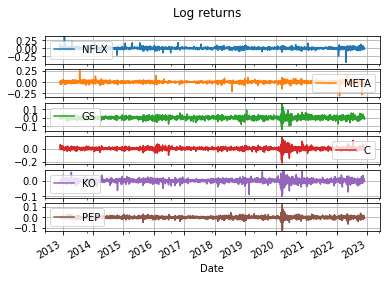
\includegraphics[width=0.5\textwidth, center]{logReturnsSubplots.png}

Possiamo subito notare come le serie dei rendimenti possano darci una diversa prospettiva sull'andamento dei titoli rispetto alla sola serie dei prezzi, infatti ci permettono di confrontare diversi titoli aventi prezzi molto differenti e quindi di concentrarci sull'andamento e non sul valore. Nel primo grafico Netlfix (blu) e Meta(arancione) sono i due titoli con piú outliers rispetto agli altri titoli e che di conseguenza hanno avuto dei movimenti di prezzo  piú ampi e forti (sia in positivo che in negativo) rispetto agli altri titoli. Inoltre nel secondo grafico si nota l'importanza che ha avuto la crisi causata dall'epidemia di covid-19 sui mercati nel 2020, tranne che nei che su Netflix e Meta. Che peró hanno avuto dei cali dopo il 2020, Netflix ad esempio aveva divulgato la notizia della perdita di abbonati alla piattaforma.
\section{Rendimenti con istogrammi}
Plottiamo ora i rendimenti tramite gli istogrammi con il seguente metodo:
\begin{lstlisting}
    plt.hist(rlNFLX, density=True, bins=50)
    plt.title('NFLX Logarithmic returns histogram')
\end{lstlisting}

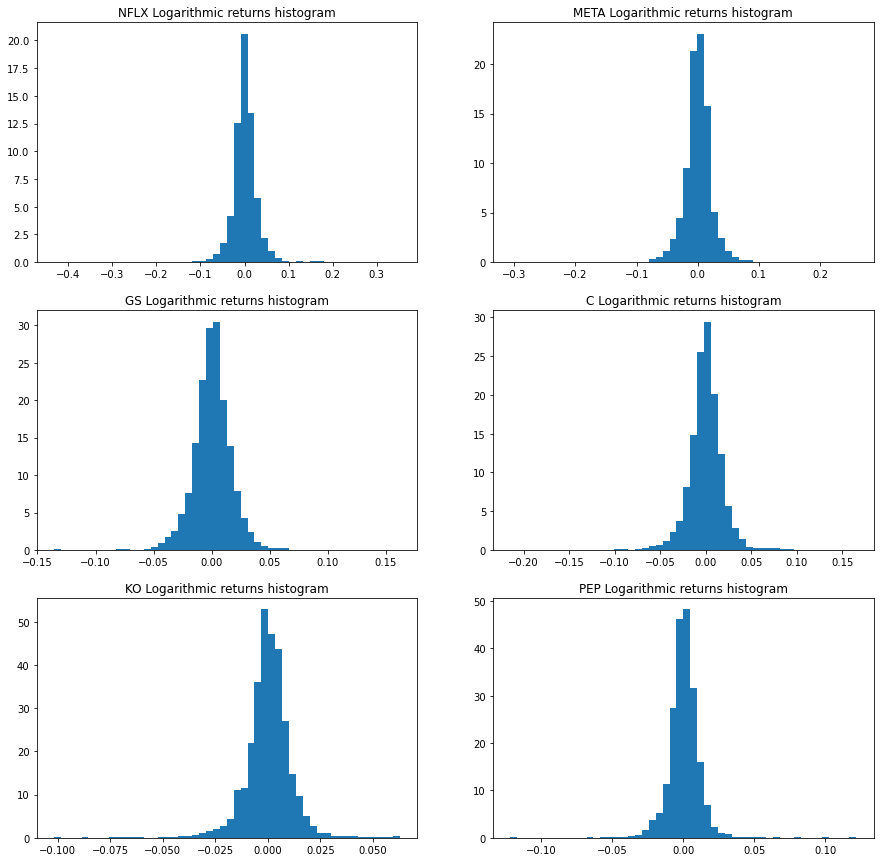
\includegraphics[width=0.5\textwidth, center]{logHist.png}
Tramite gli istogrammi possiamo valutare la quantitá di volte che si sono presentati i rendimenti nella serie, e si nota subito che per un titolo come Golden Sachs si ha un istogramma piú largo rispetto a Netflix ad esempio, questo indica una maggiore stazionarietá del titolo e di conseguenza dei cambi di prezzo piú lievi.
\section{Grafici diagnostici}
Per studiare meglio i rendimenti aggiungiamo altri 3 grafici all'istogramma, la kernel density, boxplot e qq-plot.
\begin{itemize}[leftmargin=30pt, rightmargin=2cm]
\item Box Plot -> In un solo gradico ci mostra: mediana, media primo quartile, terzo quartile e la distanza tra essi, e infine ci mostra anche gli outliers
\item QQ-Plot -> Ci mostra quanto una serie é prossima alla normalitá. Una serie normale ha la linea del qq plot esattamente in diagonale
\item Kernel density -> É una curva addolcita dell'istogramma
\end{itemize}
Il codice per produrre i grafici é il seguente:
\begin{lstlisting}[language=python]
    #NFLX
    fig = plt.figure(figsize=(15, 15))

    ax=fig.add_subplot(221)
    plt.hist(rlNFLX, density=True, bins=50)
    plt.title('NFLX Log returns histogram')
    
    ax=fig.add_subplot(222)
    plt.boxplot(rlNFLX)
    plt.title('NFLX Log returns Boxplot')
    rlNFLX.to_frame().boxplot()
    
    ax=fig.add_subplot(223)
    sm.graphics.qqplot(rlNFLX, line='s', ax=ax)
    plt.title('NFLX Log returns Q-Q plot')

    ax=fig.add_subplot(224)
    rlNFLX.plot.density()
\end{lstlisting}
Il codice soprastante é il codice per produrre i grafici di Netflix, in modo equivalente possiamo produrre i grafici per gli altri titoli.
\subsection{NFLX}
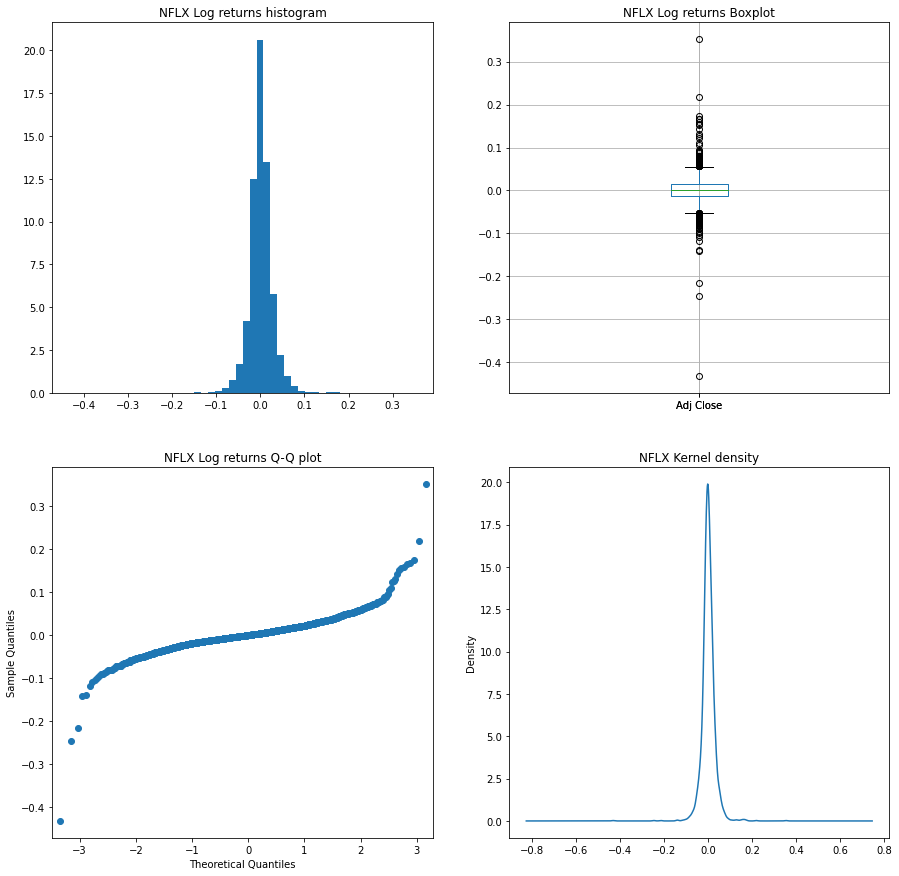
\includegraphics[width=0.5\textwidth, center]{graficiNFLX.png}
Netflix presenta una distribuzione molto compatta e ricca di outliers, come si puó vedere nel BoxPlot
\subsection{META}
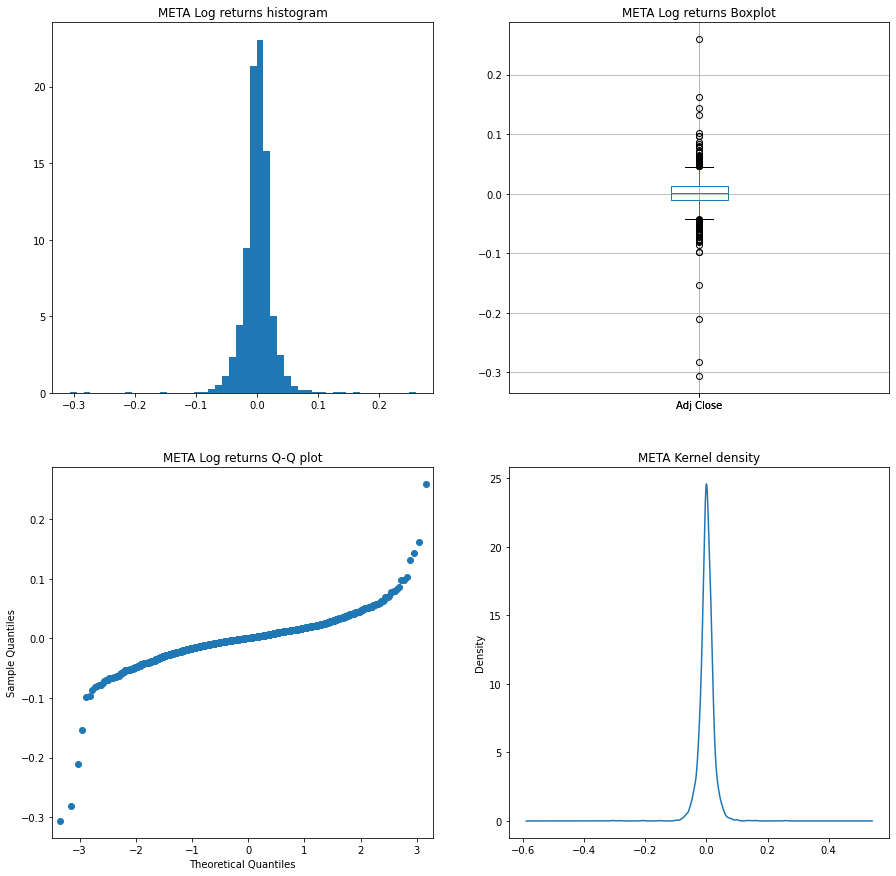
\includegraphics[width=0.5\textwidth, center]{graficiMETA.png}
Meta rispetto a Netflix ha una curva che si avvicina di piú alla normalitá ma resta comunque ricco di outliers
\subsection{GS}
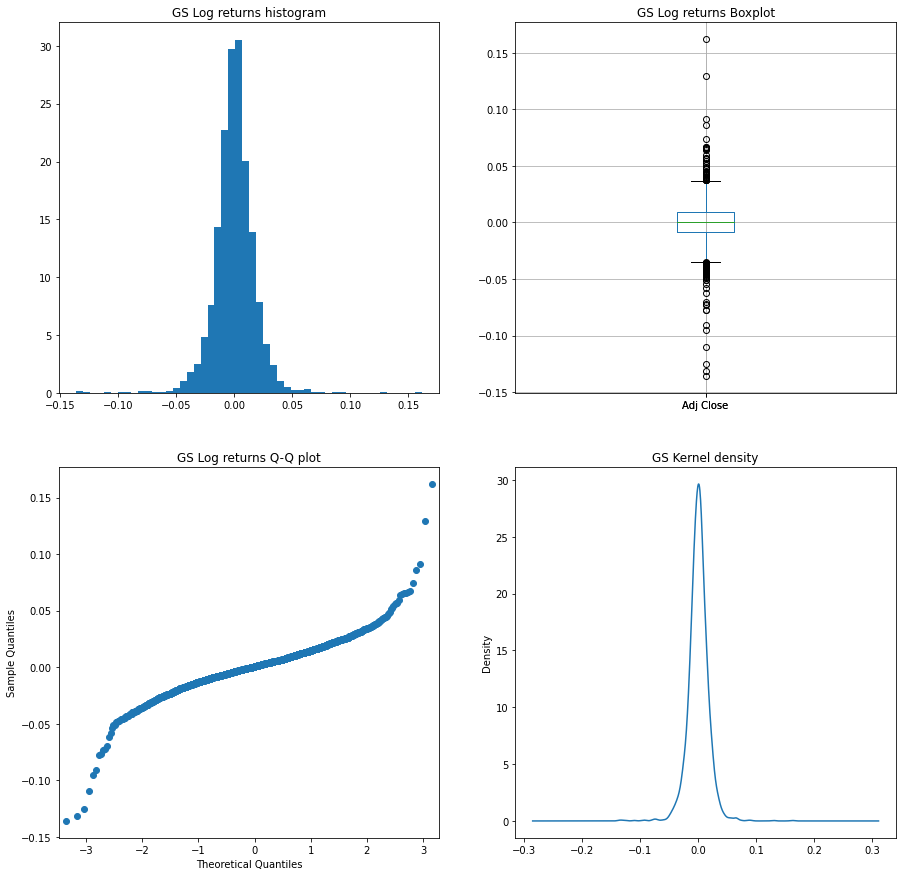
\includegraphics[width=0.5\textwidth, center]{graficiGS.png}
Goldach Sech é il titolo tra i sei che si approssima meglio ad una distribuzione normale, anche i suoi outliers sono piú equamente distribuiti
\subsection{C}
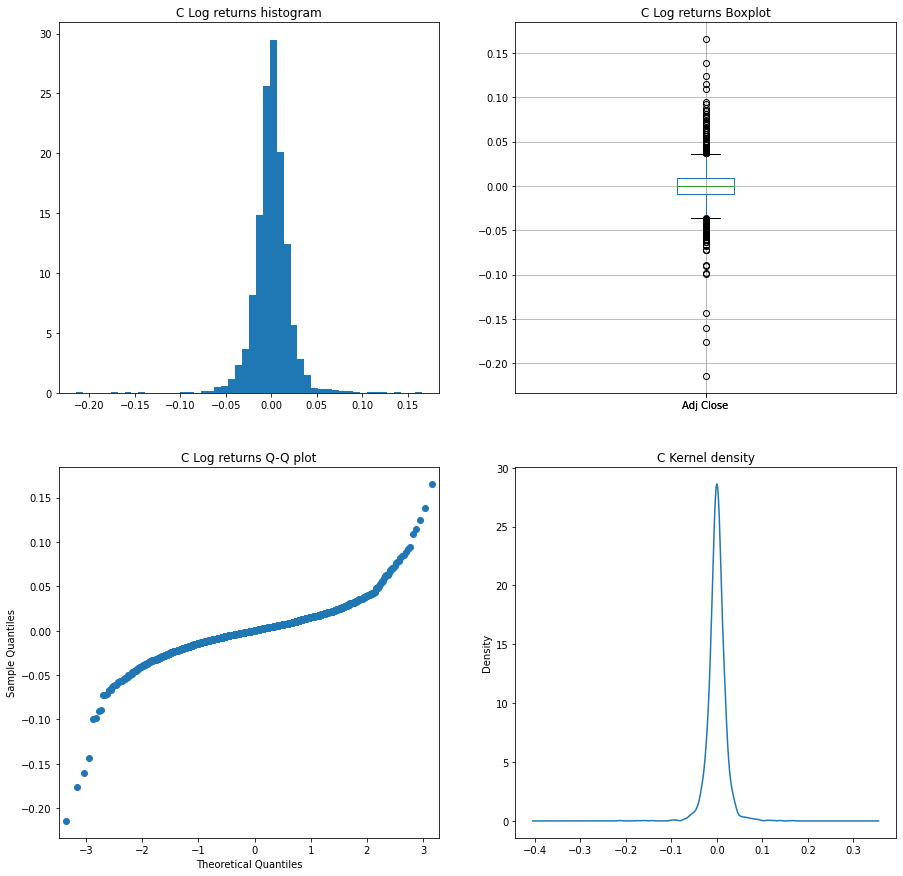
\includegraphics[width=0.5\textwidth, center]{graficiC.png}
Citigroup, come Netflix ha molti outliers distanti dalla media
\subsection{KO}
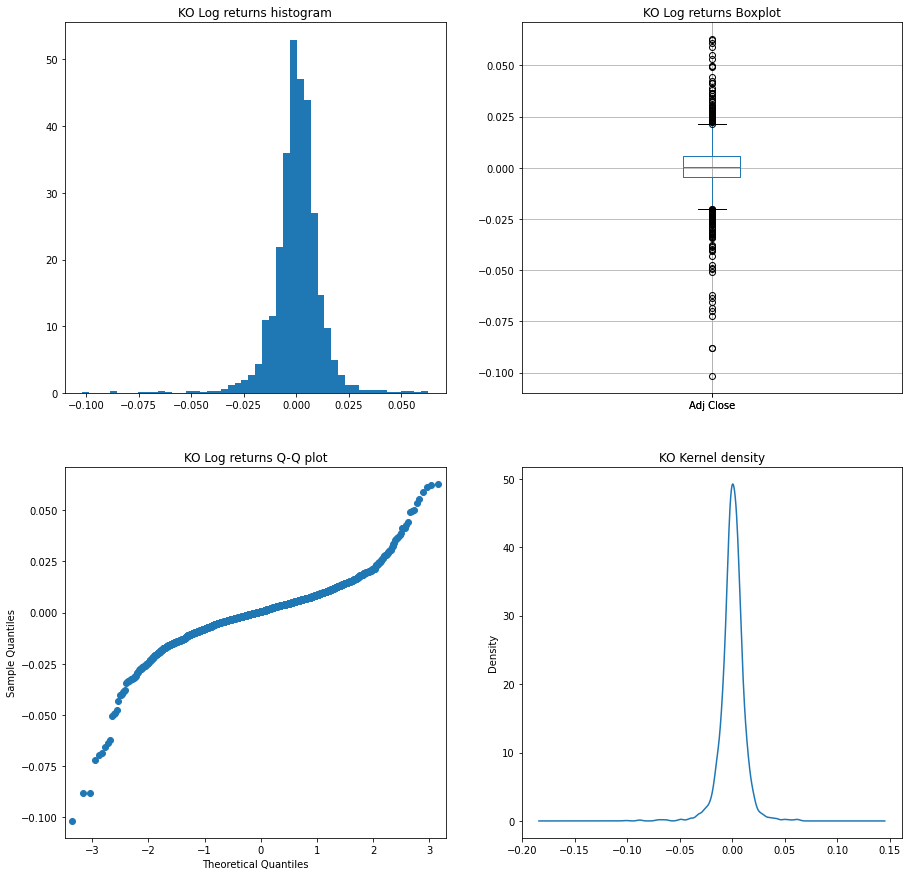
\includegraphics[width=0.5\textwidth, center]{graficiKO.png}
Coca-Cola é quello piú di tutti con un maggiore skew, infatti la distribuzione non é centrata. e presenta outliers distribuiti lungo tutto l'asse verticale
\subsection{PEP}
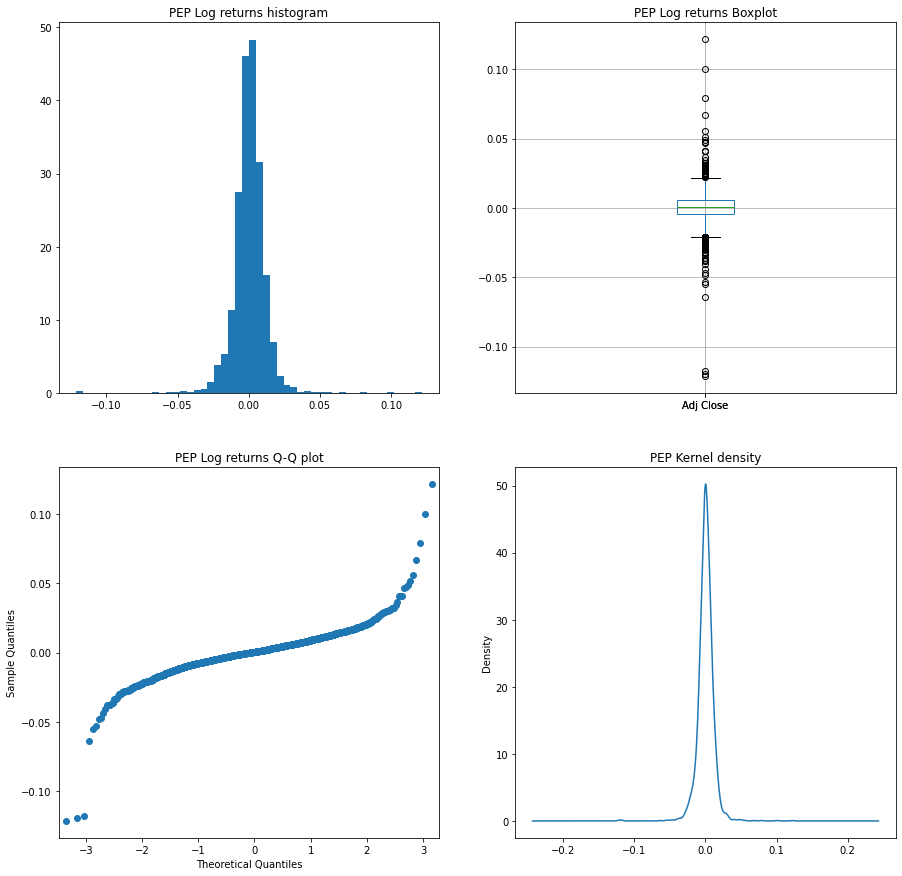
\includegraphics[width=0.5\textwidth, center]{graficiPEP.png}
Pepsi, rispetto al suo concorrente presenta la maggior parte dei suoi outliers vicini alla media e pochi lontani

\section{Statistiche descrittive univariate}
Ora procediamo con il calcolo dei seguenti dati:
\begin{itemize}[leftmargin=30pt, rightmargin=2cm]
\item Media
\item Varianza
\item Deviazione standard
\item Asimmetria
\item Curtosi
Per calcolare i dati usiamo le seguenti funzioni sulle serie:
\begin{lstlisting}[language=python]
    #NFLX
    meanNFLX = round(rlNFLX.mean(), 4)
    varNFLX = round(rlNFLX.var(), 4)
    stdNFLX = round(rlNFLX.std(), 4)
    skewNFLX = round(rlNFLX.skew(), 4)
    kurtNFLX = round(rlNFLX.kurtosis(), 4)
\end{lstlisting}
Calcolati tutti i valori li uniamo in un unico DataFrame cosi che possiamo confrontarli
\end{itemize}
\begin{tabular}{lrrrrrr}
\toprule
{} &     NFLX &     META &      GS &        C &       KO &      PEP \\
\midrule
Mean               &   0.0013 &   0.0005 &  0.0005 &   0.0002 &   0.0003 &   0.0005 \\
Variance           &   0.0009 &   0.0006 &  0.0003 &   0.0004 &   0.0001 &   0.0001 \\
Standard Deviation &   0.0300 &   0.0241 &  0.0176 &   0.0203 &   0.0115 &   0.0115 \\
Skewness           &  -0.4118 &  -1.1173 & -0.1999 &  -0.4763 &  -0.8931 &  -0.5869 \\
Kurtosis           &  31.0142 &  27.8449 &  9.8418 &  14.9718 &  10.6779 &  23.7351 \\
\bottomrule
\end{tabular}

\noindent Il titolo con il rendimento piú alto é Netflix che ha una media di \num{0.0013} mentre quello con il rendimento piú basso é Citigroup con \num{0.0002}.
Mentre per quanto riguarda la deviazione standard, il titolo piú alto é sempre Netflix con \num{0.03} mentre quelli piú bassi sono Coca-Cola e Pepsi con \num{0.0115} [...]
\section{Varianza e covarianza}
Calcoliamo ora la matrice di covarianza e la covarianza tra i nostri titoli con le seguenti funzioni:
\begin{lstlisting}[language=python]
    #Covariance Matrix
    covariance = rlMarket.cov().iloc[0,1]
    covarianceMatrix  = rlMarket.cov()
\end{lstlisting}
Che ci restituiscono per la covarianza: \num{0.0003}, mentre per la matrice:

\begin{tabular}{lrrrrrr}
\toprule
{} &      NFLX &      META &        GS &         C &        KO &       PEP \\
\midrule
NFLX &  0.000902 &  0.000298 &  0.000147 &  0.000157 &  0.000047 &  0.000068 \\
META &  0.000298 &  0.000583 &  0.000157 &  0.000164 &  0.000062 &  0.000082 \\
GS   &  0.000147 &  0.000157 &  0.000311 &  0.000296 &  0.000085 &  0.000084 \\
C    &  0.000157 &  0.000164 &  0.000296 &  0.000414 &  0.000102 &  0.000092 \\
KO   &  0.000047 &  0.000062 &  0.000085 &  0.000102 &  0.000131 &  0.000096 \\
PEP  &  0.000068 &  0.000082 &  0.000084 &  0.000092 &  0.000096 &  0.000132 \\
\bottomrule
\end{tabular}

Procediamo con il calcolo della matrice di correlazione con il seguente codice:
\begin{lstlisting}
    correlation = rlMarket.corr()
    plt.figure(figsize=(15,15))
    plt.title('Matrice di correlazione')
    sns.heatmap(correlation, vmax=1, square=True, annot=True, cmap='YlGnBu')
\end{lstlisting}

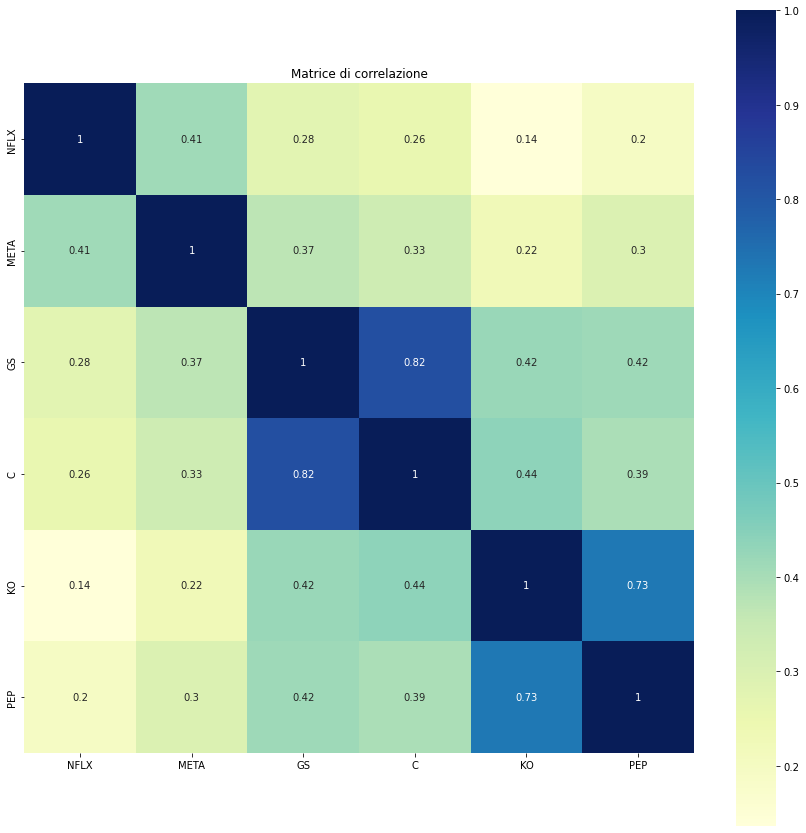
\includegraphics[width=0.5\textwidth, center]{correlationMatrix.png}

Proseguiamo quindi con la costruzione degli scatter plot
\begin{lstlisting}
    plt.figure(figsize=(15,15))
    pd.plotting.scatter_matrix(rlMarket, figsize=(12, 12))
    plt.show()
\end{lstlisting}
Con la seguente immagine:

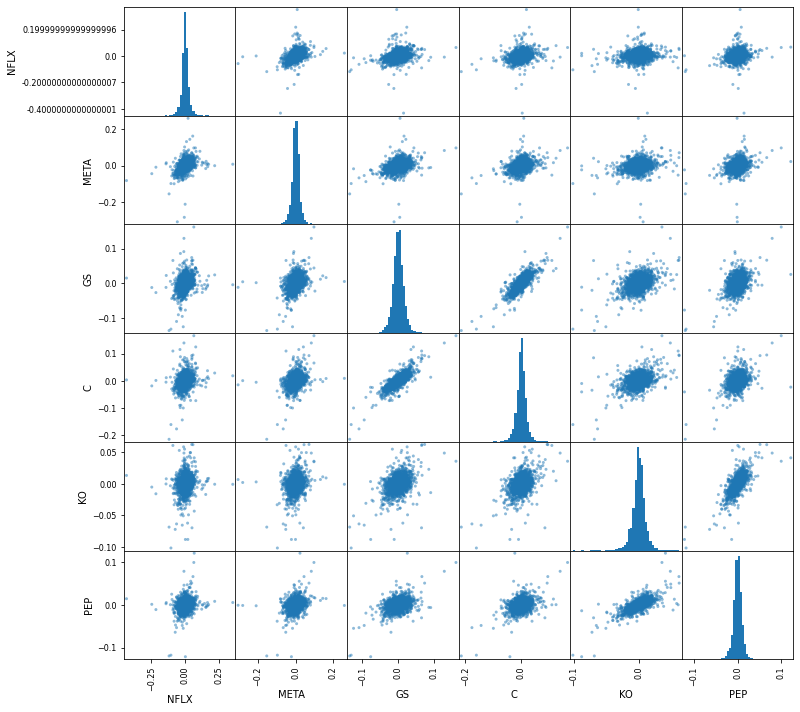
\includegraphics[width=0.5\textwidth, center]{scatterPlot.png}
[...]
\chapter{Analisi di previsione}
\tableofcontents
\end{document}